\documentclass[a4paper,14pt]{extreport}

% packages to support Cyrillic fonts, needed to write abstracts
\usepackage[T2A]{fontenc} 
\usepackage[utf8]{inputenc} 
\usepackage[russian,english]{babel}
\usepackage{csquotes}

% usual packages
\usepackage[left=30mm, right=10mm, top=20mm, bottom=20mm]{geometry}

\usepackage{graphicx} % to add figures
\graphicspath{{figures/}}

\usepackage{hyperref} % to add clickable contents menu

\usepackage[style=numeric]{biblatex}
\addbibresource{bibliography.bib}

\usepackage{blindtext}

% the following three definitions are to be changed by student
\def\myauthor{Gennady Golovkin} % author
\def\mycoach{Abel Sanchez} % coach, adviser etc.
\def\mytitle{Knockoutization of Arrogant Opponents by Nearest Neighbour Punching Algorithm} % title
%\def\mydegree{Bachelor in Computer Systems and Software}
%\def\mydegreecode{5B070400}
\def\mydegree{Bachelor in Information Systems}
\def\mydegreecode{5B070300}

% preamble ends here

\begin{document}
    % don't touch these two lines :)
    \begin{titlepage}
\begin{center}
\large
\vspace{1cm}
\begin{figure}[h]
    \centering
    
\includegraphics[scale=0.2]{figures/logoNew.png}
\end{figure}

\textbf{Suleyman Demirel University}

\textbf{Faculty of Engineering and Natural Science}

\vspace{5cm}
\huge
\textbf{\diplomaproject}

\vspace{1cm}
\normalsize
\mytitle

\vspace{1cm}
\normalsize
\begin{center}
    \textbf{Kaldybekova Diana}
    
    \textbf{Khassenova Aidana} 
    
    \textbf{Maidanbekov Dias}
    
    \textbf{Gizatov Arsen} 
\end{center}


\vspace{1cm}
\normalsize
\mydegreecode - "\mydegree"


\vfill
Kaskelen, 2022

\end{center}
\end{titlepage}
    \newpage
\pagestyle{empty}

\begin{center}
\large
Ministry of Education and Science of the Republic of Kazakhstan

Suleyman Demirel University

Faculty of Engineering and Natural Sciences

\vspace{2cm}
\textbf{\mytitle}

\vspace{1cm}
\large
A thesis submitted for the degree of

\mydegree

(degree code: \mydegreecode)

\vspace{2cm}
Author: \textbf{\myauthor}

\vspace{2cm}
Supervisor: \textbf{\mycoach}

\vspace{2cm}
Dean of the faculty:

\textbf{Assist. Prof. Meirambek Zhaparov}


\vfill
Kaskelen, 2018
\end{center}
    
    % edit abstracts
    \newpage
\pagestyle{plain}

\begin{center}
    \Large
    \textbf{Abstract}
\end{center}
There are many ready-made implementations in the world to simplify people's lives in different spheres. For example, there are many automated services in our city to simplify various life processes. If you want a quick snack, use Wolt, Glovo. Need a taxi, delivery? Install Yandex Taxi, Didi. But what if the human soul wants to do good and do charity? In practice, the fact was noticed that it was quite difficult to find points where it would be possible to donate unused things, share food and be aware of the charity actions of activists. One application could become a single center for all charitable activities. you can join various events or, conversely, announce an event. It would be possible to be aware of donations for food and clothing, or perhaps even find out which orphanages/nursing homes can be visited and helped.
    \newpage
\pagestyle{plain}

{\selectlanguage{russian}
\begin{center}
    \Large
    \textbf{Аңдатпа}
\end{center}
Әлемде адамдардың өмірін жеңілдету үшін көптеген дайын бағдарламалар бар. Мысалы, біздің қаламызда әртүрлі өмірлік процестерді жеңілдету үшін көптеген автоматтандырылған қызметтер жетерлік. Егер сіз тез тамақтанғыңыз келсе, Wolt, Glovo қолданасыз. Такси, жеткізу керек пе? Яндекс Такси, Диди қолданасыз. Бірақ егер адам жақсылық жасап, қайырымдылықпен айналысқысы келсе ше? Іс жүзінде пайдаланылмаған заттарды сыйға тартуға, тамақпен бөлісуге және белсенділердің қайырымдылық шараларынан хабардар болу өте қиынға соғады.Егерде, бір бағдарлама барлық қайырымдылық қызметтінің бірыңғай орталығы болса. Адамдар әртүрлі іс-шараларға қосыла алатын немесе, керісінше, қандай да бір іс шараны жариялай алатын. Азық-түлік пен киім-кешек садақалары туралы білуге болатын, немесе қандай балалар үйлеріне / қарттар үйлеріне баруға және көмек көрсетуге болатындығын білуге болатын мүмкіндік туады.
}
    \newpage
\pagestyle{plain}

{\selectlanguage{russian}
\begin{center}
    \Large
    \textbf{Аннотация}
\end{center}
В мире существует множество готовых программ для облегчения жизни людей в разных сферах. Например, в нашем городе существует множество автоматизированных сервисов для упрощения различных жизненных процессов. Если вы хотите быструю еду, используете Wolt, Glovo. Такси, доставка? Установить Яндекс Такси, Диди. Но что, если душа человека хочет творить добро и заниматься благотворительностью? Было очень трудно найти точки, где можно было бы пожертвовать неиспользованные вещи, поделиться едой и быть в курсе благотворительных мероприятий активистов. Одно приложение может стать единым центром всей благотворительной деятельности. Можно было бы присоединиться к различным мероприятиям или, наоборот, опубликовать какое-либо событие. Возможность узнать о пожертвованиях на продукты питания и одежду, или узнать, какие детские дома / дома престарелых можно посетить и помочь.
}
    \tableofcontents
    
    % edit your chapters
    \chapter{Introduction}\label{ch:intro}
%these sections are optional, up-to the author
\section{Motivation}
In the modern world, digital technology is one of the main factors of competitiveness. It has changed the way people work, consume and communicate. Technological revolutions are taking place in all spheres of life: medicine, education, business, etc. The need to introduce information technology solutions for charity is also one of the topical issues.

According to the data, there are 35 official funds in Kazakhstan \cite{Egov}. But there are also many charitable foundations that are not mentioned in the official website. There are a lot of funds, but why don't people know about them? 

Charity is the provision of gratuitous assistance or donations of funds with the motivation to help other people or animals. In simple words, a good deed is based on charity. Since our project focuses on charity and assistance, we began to study about the state of charity in Kazakhstan. \cite{lawRk} The result showed us that charity in the Kazakh culture has some gaps. Many who want to help – do not know how. Often people don't trust charities. Why? Because not all funds publish reports on what the funds were spent on. Since it is really difficult to track what money is being spent on. Fraud and money laundering have become seen as the basis of charitable activities. In big cities there are many fundraising points, there are some events about good deeds, but there is no information about them anywhere if it were not extensive. Why is there no single solution for all these problems?

\newpage
\section{Aims and objectives}
The main goal we were considering was that there is no centralized application in our economic environment at the moment. The main thing to pay attention to is that our application solves such global problems, as in the example of people who refuse charity because of distrust of various funds and fees. And your project is related to the registration of funds and fees according to a certain template, where they must provide the appropriate documents to identify it.

If we take a closer look at how everything is implemented at the moment, then we can understand that in Kazakhstan many donations go through grapevine. That is, as we learned earlier, we do not have a centralized application as such, and this is very difficult. After all, grapevine is not always safe and truthful, because now there are many scammers who work according to this scheme, who do not provide any supporting documents, or any substantial evidence.

Our main task was so that we could make a convenient application where, as mentioned earlier, everything was centralized. That is, an application that is convenient to use for different segments of the population of our country, where not only individual fundraising for various diseases and so on will be concentrated, but also various funds and collection points for those in material need. And we have made preferences in the direction of mobile applications, since at the moment, this is the side of development that is very popular and used. We made the site only for a part of the admin, that is, for the management staff, since by making our project in the form of a website, we would have lost a significant number of our users, since now many operations and everyday tasks are done from mobile devices.




% The first chapter is \nameref{ch:intro} chapter. It is this one that you are currently reading. It gives insight into the work done. In Chapter \ref{ch:A} we review related work and formulate the problem to solve. Chapter \ref{ch:B} is describing the solution to the problem. And in \nameref{ch:concl} chapter we conclude our conclusion.
    \chapter{Methodology}\label{ch:A}

\section{Analyze}

In order to identify and solve the information problem in charity in Kazakhstan, we conducted an analysis of trends in the development of charity. We analyzed the opinions of different people about the factors influencing the development of information opportunities in charity. As a result, we were able to identify the main criteria and opinions for improving the sphere of good deeds in the IT of the future.

For clarity, we have formulated 3 main trends that should be guided in the analysis in order to get the main ideas related to charity and the solution of functionality and application development.

\begin{itemize}
    \item \textbf{Qualitative research}
    \item \textbf{Quantitative research}
    \item \textbf{Competitive analysis}
\end{itemize}

Each analysis has its own conclusions and results. Research has provided an opportunity to lay a solid foundation for the development of our ideas and beliefs. After the conducted research, we can confidently talk about what needs to be done and what is the right decision.

For proper analysis, we had to choose one of the types of marketing research. We have chosen two types of research.

1. Primary research
Whenever a study is conducted by itself or on its own behalf and it is necessary to create data to solve a specific problem, this is called primary market research. Interviews, surveys and analyses are an example of this. The primary research is considered to be a Qualitative, Quantitative research

2. Secondary research
When it uses already existing data, for example, collected by other companies and organizations, we can conduct secondary market research.
For example, third-party sources such as articles, technical documents, reports and industry statistics. Competitive research can be quoted as an example of secondary research.


\subsection{Qualitative research}

(Interviews or open questions, etc. The results are expressed in words, not numbers and graphs. This type of research is used to understand the underlying causes, opinions, and motivations.)

We interviewed 3 potential users, and also added open questions 
to the survey to understand what problems they face when they want to do charity work. 
Main question was:
\begin{itemize}
    \item In your opinion, why is it important to do charity work?
    \item Are you involved in charity, if so, how do you prefer to help?
    \item What do you think about charity in Kazakhstan?
    \item What exactly most often prevents you from doing charity work?
    \item If there was an app for various kinds of charity activities, what would you like to see in the app?
\end{itemize}

This type of analysis helped us to understand what prevents us from doing charity work and what solutions are needed to solve their problem

When the respondents were asked about charity in Kazakhstan, they were inclined to believe that charity itself is only developing in our country and people are helping each other in a difficult situation, but agreed that there is some frustration in the process, like fraud in fees. One respondent (male, 29 years old) noted some points for solving problems in fees:

- "If there is a single application for charity, what functions would you like to see?"

- “I want to see in this application how it was recorded that the person who opened the collection for a sick person had correct documents that prove the symptoms of the disease. This would be one of the solutions to the reliability of the collection and distrust of charitable collections.”

Another respondent (a woman, 28 years old) answered the same question, noting that monitoring of the collection is necessary for reporting:

- "If there was such an application, for example, I transfer some amount of money, then I would like to see its movement, that is, where this money was redirected?! It would also be possible to see active funds and fees that need not only financial issues and, for example, things or products. If there are such functions, then it would be a good application."

It is clear from the answers that people want reliability and reports on charitable collections.

\subsection{Quantitative research}

(Polling, voting, closed questions, etc. The results are expressed in numbers and statistics. This type of research is used to test or confirm hypotheses or assumptions by quantifying certain variables.)

For qualitative analysis, we conducted an online survey using Google Forms to identify any patterns and similarities in what potential users might want. A total of 50 people responded. Main question was:
\begin{itemize}
    \item How often do you do charity work? 
    \item What problems do you face when donating money for charitable purposes?
    \item Do you give things to charity, to those in need? (Clothing, shoes, etc.) 
    \item Would you use the app for various kinds of charitable activities?
    \item What would you like to see in the app?
\end{itemize}

\begin{figure}[h]
    \centering
    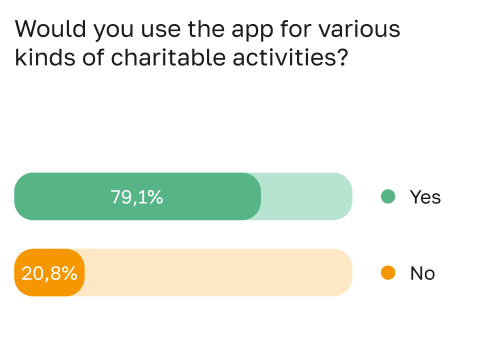
\includegraphics[width=6cm]{figures/Questionaire9.png}
    \caption{Would you use the app for various kinds of charitable activities?}
    \label{fig:4}
\end{figure}

The quantitative method is applied at all stages of work on the product. The survey makes it possible to evaluate objects and phenomena quantitatively: to understand the composition of the audience of the product, to estimate the frequency of occurrence of a certain feature, to prioritize ideas and problems, to choose the best option, etc

Quantitative data is always represented by numbers. They can be processed by statistical methods and get some specific indicators. For example, after the survey, it can be understood that almost 80\% of users want there to be a single application for charitable activities. After the survey, a common understanding of the problems that ordinary people face in good deeds was revealed. For example in the question \textit{"What problems do you face when donating money to charity?"} 25\% of the answer was about fraud, 20\% of the answer was distrust of certain fees, 20\% of the answers were problems with reports from charity fees. 

From this we can draw a conclusion and make a functional solution to these problems in our applications. The survey has predictive power, that is, it makes it possible to predict the opinions of a large number of people — the general population. The survey provides an opportunity to identify ideas for solving problems, as a result, evaluate the idea in the audience of the product. With the help of the question \textit{"Do you give things to charity, to those in need?" (Figure 2.2)} we wanted to introduce functionality about providing information on the collection point and find out the opinion of the audience. As a result, it turned out that the majority supported the idea and the functionality can be confidently added to the project.

\begin{figure}[h]
    \centering
    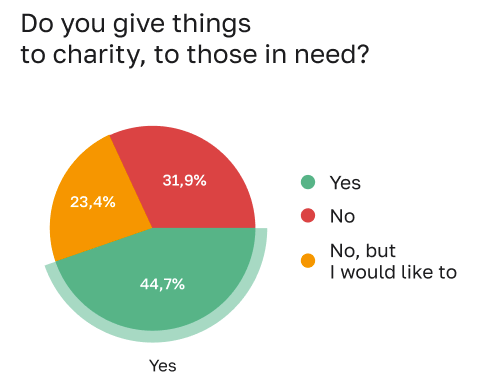
\includegraphics[width=6cm]{figures/Questionaire8.png}
    \caption{Do you give things to charity, to those in need?}
    \label{fig:2}
\end{figure}
\begin{figure}[h]
    \centering
    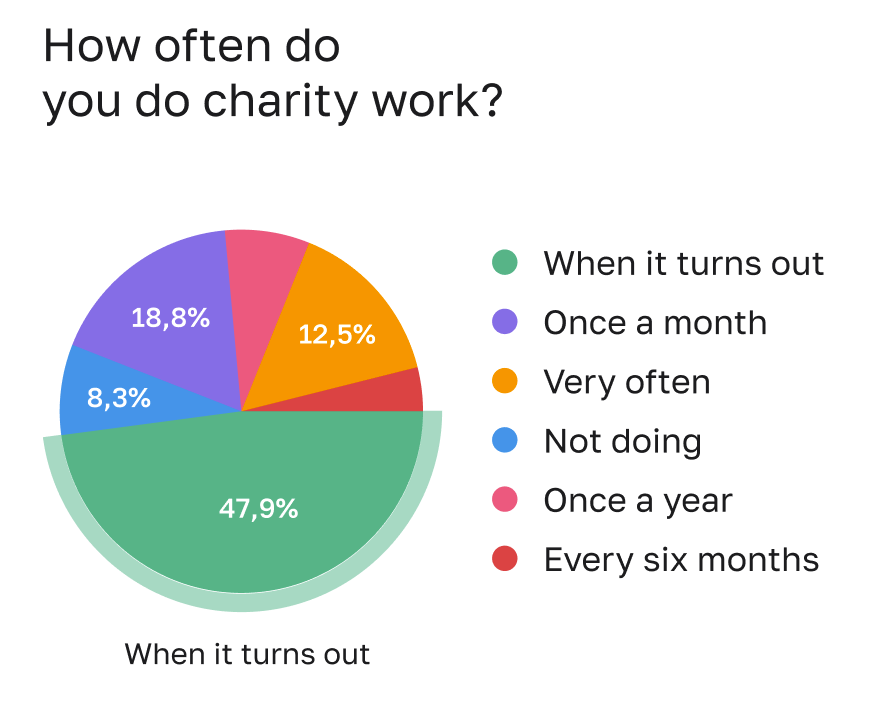
\includegraphics[width=6cm]{figures/Questionaire1.png}
    \caption{How often do you do charity work?}
    \label{fig:3}
\end{figure}

\subsection{Competitive analysis}

(A type of research through which an enterprise develops its own strategy for promoting products to the market, taking into account those features and behaviors that competitors have)

One of the most important analyses that helped us assess the competitiveness of our project. \cite{marketResearch} After all, every project operates in a competitive market. And to form a strategy, you need to take into account the specifics of the product or service, as well as understand those external factors that directly or indirectly affect the development of the project. One of the advantages of competitive analysis is to first study what and how competitors have already done, prevent their mistakes and make it better, as well as generate new ideas for the project. The analysis helped to understand that there are many projects on the market that correspond to our ideas and currently attract customers and offer some unique advantage, create value for our project.Our competitive analysis consisted of 3 stages:
\begin{enumerate}
    \item \textit{Make a list of similar projects.} 
    
        As a result of the search, there were many similar projects, but we identified only those projects that more or less fit our ideas:
        \begin{itemize}
            \item \textbf{Share The Meal} is a charity application from the World Food Program that allows you to feed children in need with a single touch of the screen. As the world faces a record number of emergencies, hunger levels are rising.
            \item \textbf{Give life} is the official application of the Gift of Life Foundation. It tells about the work of the foundation and projects. You can choose what kind of help you want to provide: subscribe to monthly donations, become a donor or volunteer. For the convenience of users, Google Play and Apple Pay are implemented in the application. Not so long ago, the mobile application of the Gift of Life Foundation took second place in the nomination "State and Society" of the Runet Rating award.
            \item \textbf{Pomosh} is the world's first mobile application of targeted and transparent help. The project is like an assembly point of a new time, uniting generations. The first target group for targeted assistance is the elderly.
            \item \textbf{Food drive} - providing targeted assistance with products. In the application, you can get acquainted with the database of promotions, addresses of participating stores and choose any place, branch, date and type of assistance you like. You can make both a one-time purchase of products and regular donations. Usually these are food packages priced from 150 rubles to 2 thousand rubles. Through Food Drive, you can also feed stray cats and dogs - this is enough to buy food.
            \item \textbf{Gofundme} is the largest crowdfunding application and a reliable leader in online fundraising. With reliable functionality, you can confidently make a donation to charity fees
        \end{itemize}
        
        
    
    \item \textit{Conduct a comparative analysis of projects} 
    
        For a comparative analysis of the product, we selected 3 projects that are more suitable for use in logic and functionality and identified the key advantages and disadvantages of each project.
        
        
        
        \begin{itemize}
            \item \textbf{Share The Meal} 
            
                Advantages:
                \begin{itemize}
                    \item The app rise money for food donation
                    \item The app feeds the childrens all around the world
                \end{itemize}
                Disadvantages:
                \begin{itemize}
                    \item The app collects money only for products
                    \item No fundraising for Kazakhstan
                    \item You can’t donate food or stuffs
                \end{itemize}
                
            \item \textbf{Gofundme}
                
                Advantages:
                \begin{itemize}
                    \item The app rise funds
                    \item Helps people around the world with fund rising
                \end{itemize}
                Disadvantages:
                \begin{itemize}
                    \item You can’t donate food or stuffs
                    \item No fundraising for Kazakhstan
                    \item Anyone can open a fundraiser there is a risk of fraud
                \end{itemize}
                
            \item \textbf{Give life}
                
                Advantages:
                \begin{itemize}
                    \item The app rise funds
                    \item There is a monthly subscription
                    \item You can apply for volunteering/donation
                \end{itemize}
                Disadvantages:
                \begin{itemize}
                    \item Inconvenient interface
                    \item No fundraising for Kazakhstan
                    \item The application will offer one fund, there is no way to help another fund
                \end{itemize}
        \end{itemize}
        
        
        
    
    \item \textit{Determining the positioning of all projects} 
    
        At this stage of the analysis, we positioned the projects of each competitor, depending on the perception of users, and this is based on the following criteria:
        \begin{itemize}
            \item popular - less popular
            \item specialized - multi functional 
        \end{itemize}
        The analysis graph (Figure: Project positioning) shows that Give Life is a one of the popular and multi functional application. And the functionality is more suitable for our project
        
        \begin{figure}[h]
            \centering
            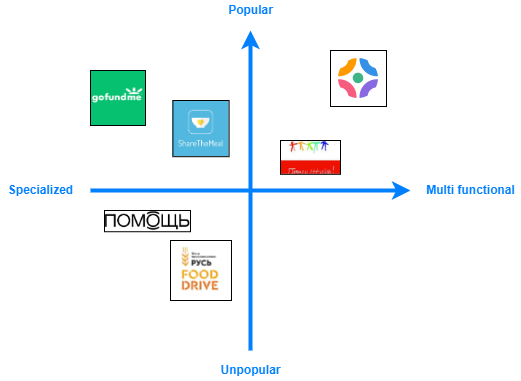
\includegraphics[width=16cm]{figures/Competitor analyze.png}
            \caption{Project positioning}
            \label{fig:1}
        \end{figure}
\end{enumerate}

\section{Research result}
Summing up the above, we were able to identify obvious problems in the environment and new ideas for the project. In the process of joint work, the conditions for the formation of the following elements of project activity have been implemented. Key insights from the research:

\begin{itemize}
    \item Lots of unreliable fundraising charities
    \item Lack of awareness of assistance opportunities
    \item Non-transparency of the activities of organizations
    \item The formal existence of most charitable foundations
    \item Not enough full reporting and monitoring from fees
    \item Difficulty to donating money to fund raises 
    \item There are no apps for charitable activities in our region
\end{itemize}

Charity is an indicator of the degree of development of society and the country as a whole. According to the results of the analysis, he showed that the culture of good deeds in our country is only developing. Currently, the number of unofficial charitable foundations and fees is growing. This at the same time led to distrust, fraud in fees. People want to do charity work, but there is no application on the market that would satisfy the needs of the user. To solve these problems, we have created a common solution by creating a single application for charitable activities.
    \chapter{BBBBB}\label{ch:B}

\section{B one}
Gennady Gennadyevich Golovkin is a legendary middle weight boxer (see Figure \ref{fig:ggg})

\begin{figure}[h]
    \centering
    
\includegraphics[scale=0.7]{ggg}
    \caption{Triple G}
    \label{fig:ggg}
\end{figure}

\section{B two}

\section{B three}
    \chapter{CCCCC}\label{ch:C}
\section{C one}
Monkey is a beast that can jump. See Appendix \ref{app:B}.
\section{C two}
\section{C three}
    \chapter{Conclusion}\label{ch:concl}
Everything is great, but there is a space for future work.
    
    \appendix
    \chapter{AppendixATitle}\label{app:A}
\section{Theorem}
\section{Proof}
etc. etc.

    \chapter{AppendixBTitle}\label{app:B}
Five little monkeys are jumping on the bed.


    \printbibliography[heading=bibintoc,title={References}]
\end{document}
